
\section{Site management}\label{sitemanagement}

Het hoofdstuk \emph{Site management} omschrijft alle relevante aspecten van het beheer van de website. Hieronder valt bijvoorbeeld het \emph{menu} en \emph{subsite management}.

\subsection{Nieuwe (lege) pagina}\label{nieuwepagina}
Het aanmaken van een nieuwe pagina is nodig om een pagina op te bouwen uit Felixblokken. Denk heir bijvoorbeeld aan een nieuwsoverzicht- of smoelenboekpagina.

\textbf{Nieuwe pagina}

\begin{itemize}
\item Ga naar \drupalpath{admin/structure/empty-page/add} (rol: beheerder) en maakt een nieuw pad aan voor de nieuwe pagina. Titel mag leeg gelaten worden. Probeer bij het aanmaken van het pad zoveel mogelijk de menustructuur te volgen. Maak je een pagina onder wonen-en-leven aan, vul dan \emph{wonen-en-leven/nieuwepagina} in.
\item Na opslaan kom je op de overzichtslijst van alle lege pagina URL's. Ga nu naar de zojuist aangemaakt url toe. Dat kan via dit overzicht of door de URL in de browser in te typen.
\item Je komt nu op een lege pagina uit met alleen Felix regio's. Je kan nu elke regio vullen met een blok waar nodig. Zie \emph{Felix}\seeone{felix} voor een overzicht van Felixblokken.
\end{itemize}

\textbf{Koppelen aan een menu}
Om de pagina in een menu te zetten volg je de volgende stappen.

\begin{itemize}
\item Bewerk het hoofdmenu. Zie \emph{Menu}\seeone{menu} voor het bewerken en aanmaken van menuitems.
\item Voeg een nieuwe link toe.
\item Voeg een titel toe en vul de URL van de zojuist aangemaakte pagina op.
\item Kies bij Bovenliggend onderdeel waar deze pagina in de structuur terecht moet komen.
\item Sla op. Je komt nu terug op de lege pagina. Wanneer er menuitems zijn op hetzelfde niveau zal het submenu zichtbaar worden aan de linkerkant.
\end{itemize}
\subsection{Nieuwe peiling}\label{nieuwepeiling}
In deze paragraaf zal stap voor stap beschreven worden hoe je een \emph{peiling} aanmaakt en toont op de website.

\textbf{Nieuwe peiling aanmaken}

\begin{enumerate}
\item Ga naar \drupalpath{node/add/poll}
\item Vul een vraag in bij het veld \emph{Vraag}.
\item Vul minstens twee mogelijke antwoorden in bij het veld \emph{Keuze}, klik op de knop \emph{Meer keuzes} om meerdere keuzes te specificeren.
\item Bepaal bij het veld \emph{Peilingsstatus} of de Peiling \emph{gesloten} of \emph{actief} is.
\item Selecteer hoe lang de Peiling moet duren bij het veld \emph{Peilingsduur}.
\item Specificeer optioneel een locatie bij de velden onder \emph{Locatie}.
\item Klik onderaan de pagina op de knop \emph{Opslaan} om de inhoud op te slaan.
\end{enumerate}

\begin{center}
	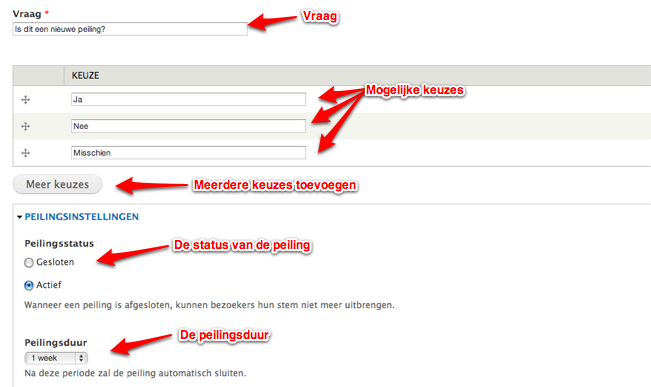
\includegraphics[width=\textwidth]{img/peiling_1.png}
\end{center}


\textbf{Nieuwe peiling tonen}

\begin{enumerate}
\item Ga naar de gewenste pagina waarop je peiling wil tonen.
\item Klik in de gewenste \emph{regio} op het \emph{tandwieltje} en klik vervolgens op \emph{Blok toevoegen}
\end{enumerate}

\begin{center}
	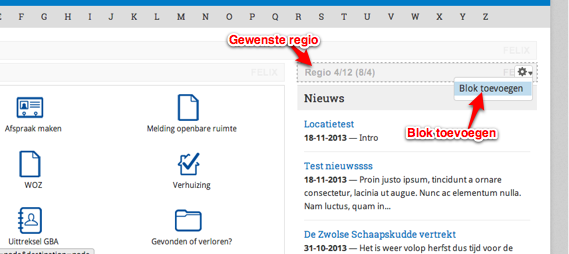
\includegraphics[width=\textwidth]{img/peiling_2.png}
\end{center}

Nadat je op het \emph{tandwieltje} hebt geklikt, zal een overzicht verschijnen welke je kunt zien in de onderstaande afbeelding.

\begin{center}
	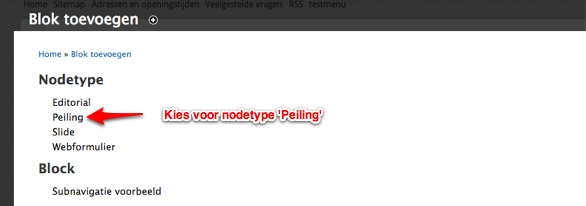
\includegraphics[width=\textwidth]{img/peiling_3.png}
\end{center}

\begin{enumerate}
\item Klik onder het kopje \emph{Nodetype} op de link genaamd \emph{Peiling}.
\item Vervolgens kun je de weergavemodus kiezen, kies voor \emph{Volledige inhoud}.
\item Nadat je op \emph{Volledige inhoud} hebt geklikt, krijg je een lijst te zien met alle bestaande peilingen, klik op de gewenste peiling. De peiling zal daarna direct toegevoegd worden aan de gewenste regio.
\item Indien je de peiling wilt verplaatsen binnen de gekozen regio, raadpleeg dan \emph{Felix blok volgorde aanpassen} \seeone{felixblokvolgorde}
\end{enumerate}


\section{Menu}\label{menu}
Via een aparte sectie in de beheeromgeving kunnen de beschikbare menu's worden aangepast. Het menu systeem staat in Drupal los van de inhoud (nodes). Om een pagina in het menu toe te voegen zal eerst de pagina toegevoegd moeten worden en kan daarna het menu-item worden aangemaakt.

\subsection{Menu-items toevoegen}\label{menuitemstoevoegen}
menu items toevoegen tekst

\subsection{Menu-items bewerken}\label{menuitemsbewerken}
menu items bewerken tekst
\subsection{Nieuwsbrief}
\pvelist{ \pve{4.25} }

De module ProRail Newsletter maakt gebruik van Drupal webforms voor het aanbieden 
van in- en uitschrijfformulieren voor nieuwsbrieven. Elke nieuwsbrief heeft 
\'{e}\'{e}n aanmeldformulier en \'{e}\'{e}n afmeldformulier. Aanmeldingen zijn 
eenvoudigweg inzendingen van de aanmeldformulieren. Er wordt niet voorzien in een 
koppeling naar een backendsysteem voor verzending, aanmeldingen dienen handmatig 
gedownload te worden als CSV-bestand (zie sectie \ref{sec:inzienaanmeldingen}). 
De module vult de webformulieren op twee belangrijke punten aan:

\begin{itemize}
\item Er wordt per aanmelding een uniek \emph{token} (een tekenreeks van 
willekeurige tekens) aangemaakt, dat meegestuurd moet worden in de 
bevestigingsemail (hiertoe moet de waarde van het tokenveld expliciet in de emailtemplate worden opgenomen) en er wordt in een bevestigingspagina voorzien, waarin 
het token verwerkt wordt en bij een juist token het veld \emph{Bevestigd} bij de aanmelding op 
\emph{Ja} wordt gezet (zie sectie \ref{sec:vereistenaanmeldformulieren}).
Op deze wijze is het niet mogelijk om een email-adres aan te melden via het 
formulier zonder toestemming van degene die werkelijk toegang heeft tot het 
email-adres. 
\item Bij het invullen van een afmeldingsformulier worden aanmeldingen voor het opgegeven 
email-adres (d.w.z. inzendingen van het bijbehorende aanmeldformulier) verwijderd.
\end{itemize}

\subsubsection{Standaard oplevering}
Bij oplevering is er als voorbeeld voorzien in twee aanmeldformulieren en een 
afmeldformulier. Het formulier \emph{Aanmelden nieuwsbrief} is ook daadwerkelijk 
geconfigureerd als aanmeldformulier, het formulier \emph{Aanmelden nieuwsbrief 
eenvoudig} is uitsluitend ter voorbeeld. Het afmeldformulier is gekoppeld aan 
het formulier \emph{Aanmelden nieuwsbrief}.
Afmeldingen kunnen, maar hoeven niet bekeken te worden; ze worden automatisch 
verwerkt, mits voldaan is aan de voorwaarden voor aan- en afmeldformulieren 
zoals hieronder opgesomd.  

\subsubsection{Inzien aanmeldingen}
\label{sec:inzienaanmeldingen}
Als voorbeeld bekijken we hoe de aanmeldingen voor de nieuwsbrief van het 
formulier \emph{Aanmelden nieuwsbrief} ingezien kunnen worden (dit is standaard webform-functionaliteit 
en werkt dus ook voor willekeurige andere webformulieren).

1. Zoek het formulier, bijvoorbeeld via de tab Webformulieren onder Inhoud
\begin{center}
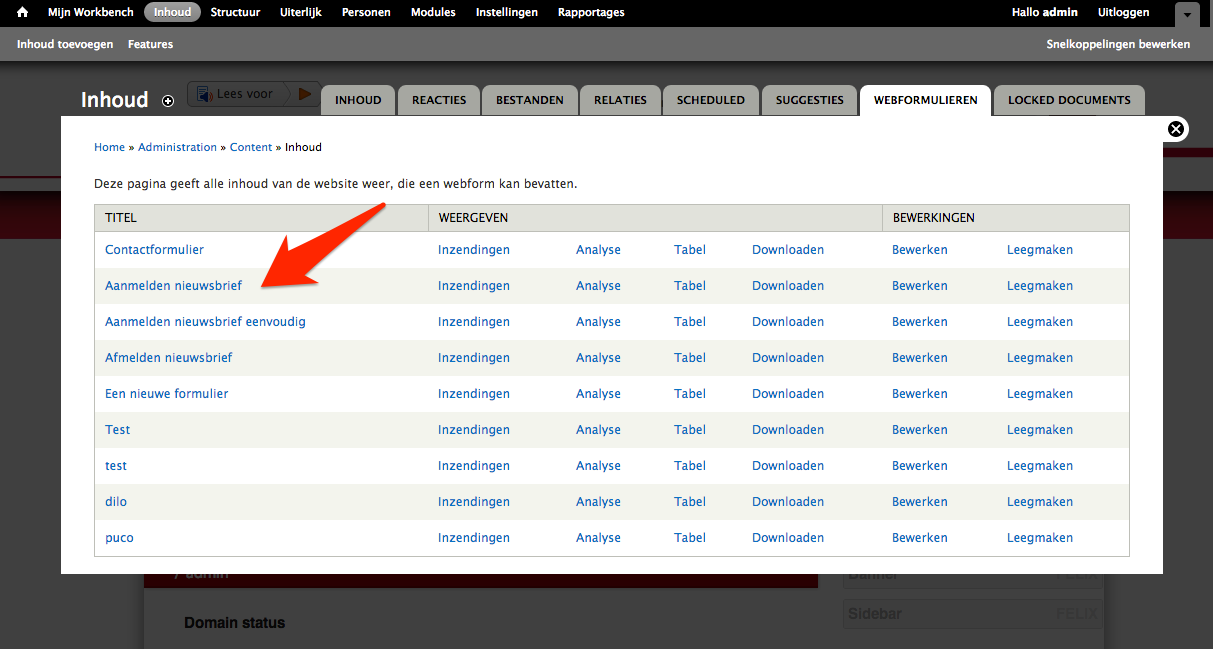
\includegraphics[width=\textwidth]{img/nieuwsbrief/form_aanmelden_nieuwsbrief.png}
\end{center}

2. Klik op de link Tabel
\begin{center}
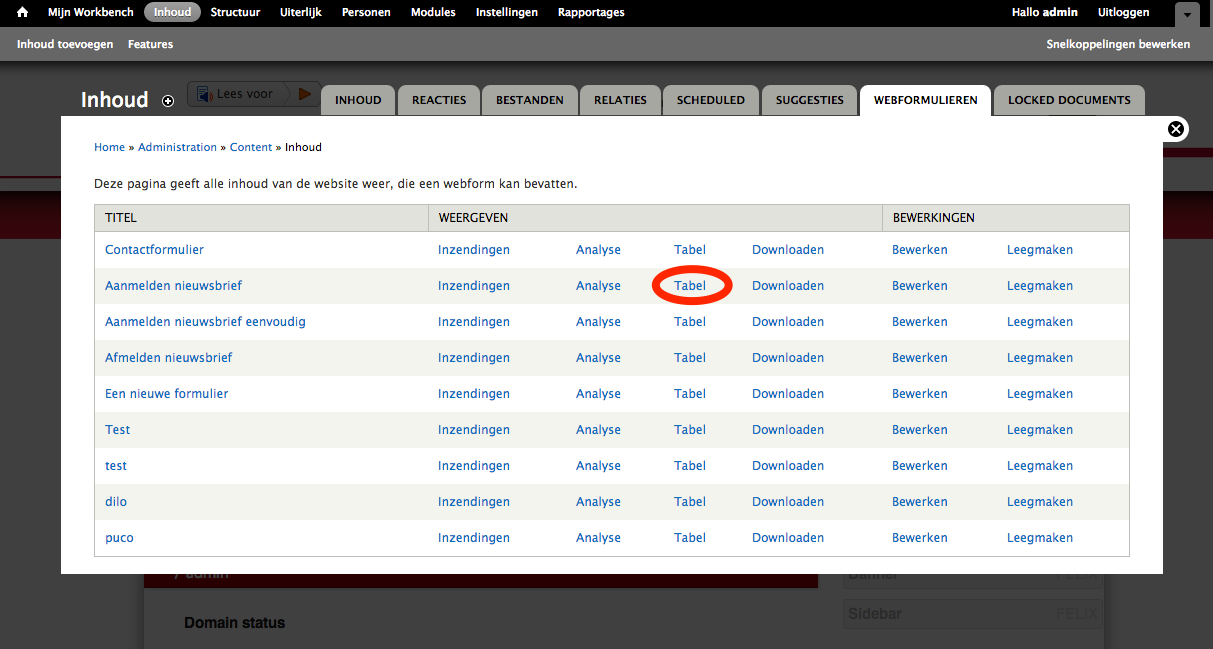
\includegraphics[width=\textwidth]{img/nieuwsbrief/aanmelden_nieuwsbrief_tabellink.png}
\end{center}

3. Een tabel met inzendingen verschijnt.
\begin{center}
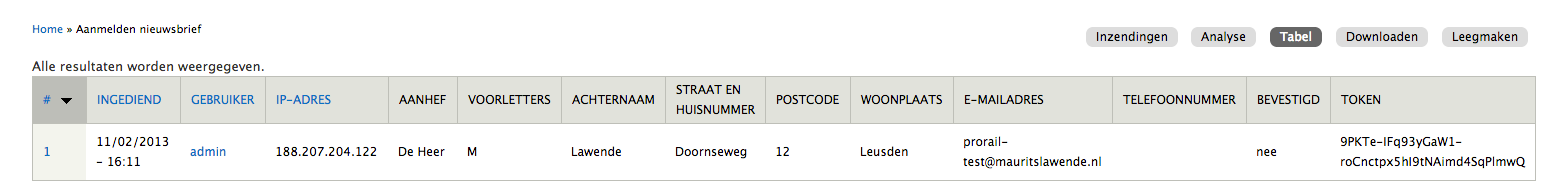
\includegraphics[width=\textwidth]{img/nieuwsbrief/aanmelden_nieuwsbrief_inzendingen.png}
\end{center}

4. De inzendingen kunnen gedownload worden als CSV-bestand op de link Download
\begin{center}
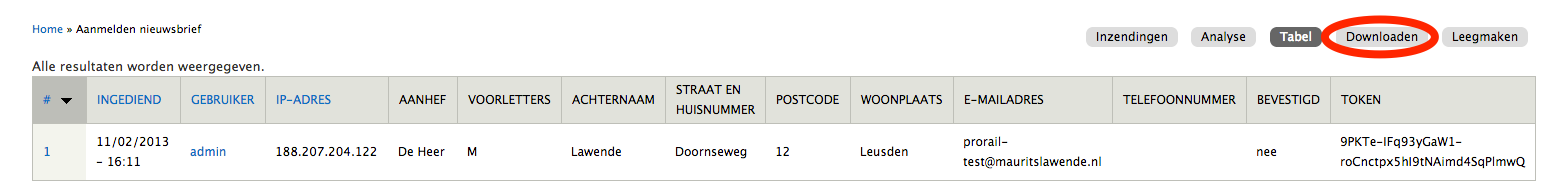
\includegraphics[width=\textwidth]{img/nieuwsbrief/aanmelden_nieuwsbrief_download.png}
\end{center}

Op dit scherm zijn een aantal instellingen mogelijk met bestrekking tot het te 
genereren export-bestand, zoals het scheidingsteken tussen waardes, welke waardes 
ge\"{e}xporteerd moeten worden en welke inzendingen gedownload moeten worden, zoals 
alleen nieuwe inzendingen, alle inzendingen, of een specifiek aantal inzendingen.

\textbf{Let op:} De download bevat alle aanmeldingen, inclusief de 
onbevestigde aanmeldingen. Het is dus bij verdere verwerking van het 
export-bestand van belang dat onbevestigde aanmeldingen worden uitgefilterd 
(dat zijn dus de aanmeldingen waarbij de kolom \emph{Bevestigd} niet op 
\emph{ja} staat).

N.b. Op het download-scherm kan gekozen worden voor het bestandsformaat 
\emph{Microsoft Excel}. Deze optie kan beter niet gebruikt worden, want de enige 
aanpassing die aan het gegenereerde bestand wordt gedaan is het veranderen van de 
bestandsnaamextensie in 
xls. De inhoud van het bestand blijft gelijk, waardoor het geen valide XLS-bestand is.

\subsubsection{Vereisten aanmeldformulieren}
\label{sec:vereistenaanmeldformulieren}
Aanmeldformulieren kunnen als normale webformulieren worden aangemaakt, mits ze aan 
een aantal eisen voldoen (op deze vereisten is geen actieve controle bij het selecteren 
van het formulier in de beheer-interface).

\begin{itemize}
\item Een veld met de machinenaam \emph{email}, dat het aangemelde email-adres bevat. Dit dient een veld van het type \emph{email} te zijn;
\item Een \emph{verborgen} veld met de machinenaam \emph{bevestigd}. Hiervoor moet 
de instelling \emph{veilige waarde} gebruikt worden zodat de 
waarde niet van buitenaf meegestuurd kan worden door middel van een malafide inzending. 
De standaard-waarde van dit veld moet op \emph{nee} ingesteld worden (in feite 
zijn hier geen beperkingen op anders dan dat de standaard-waarde niet \emph{ja}
mag zijn, want dat is de waarde die door de module wordt ingevuld bij bevestiging van 
de inschrijving).
\item Een \emph{verborgen} veld met de machinenaam \emph{token}. Dit veld wordt gebruikt voor het opslaan 
en controleren van het aangemaakte token. 
Ook hiervoor dient de instelling \emph{veilig waarde} gebruikt te worden. De 
standaard-waarde hoeft niet ingesteld te worden.
\item Een bevestigingsemail voor de gebruiker met daarin een bevestigingslink. De 
be\-ves\-ti\-gings\-link heeft de volgende vorm:
\url{http://www.prorail.nl/nieuwsbrief/bevestigen/\%value[token]}
Het voorbeeldformulier \emph{Aanmelden nieuwsbrief} bevat ook een voorbeeld van 
de bevestigingsemail met de token op de juiste manier erin opgenomen.
\end{itemize}

Naast deze velden kunnen eventueel andere velden naar keuze worden toegevoegd. Zo 
heeft het standaard opgeleverde aanmeldformulier velden voor postadres-gegevens. 
Aangeraden wordt om zo min mogelijk informatie van de gebruiker te vragen, zodat 
de drempel om voor een nieuwsbrief aan te melden zo laag mogelijk is.

\begin{figure}[p]
\centering
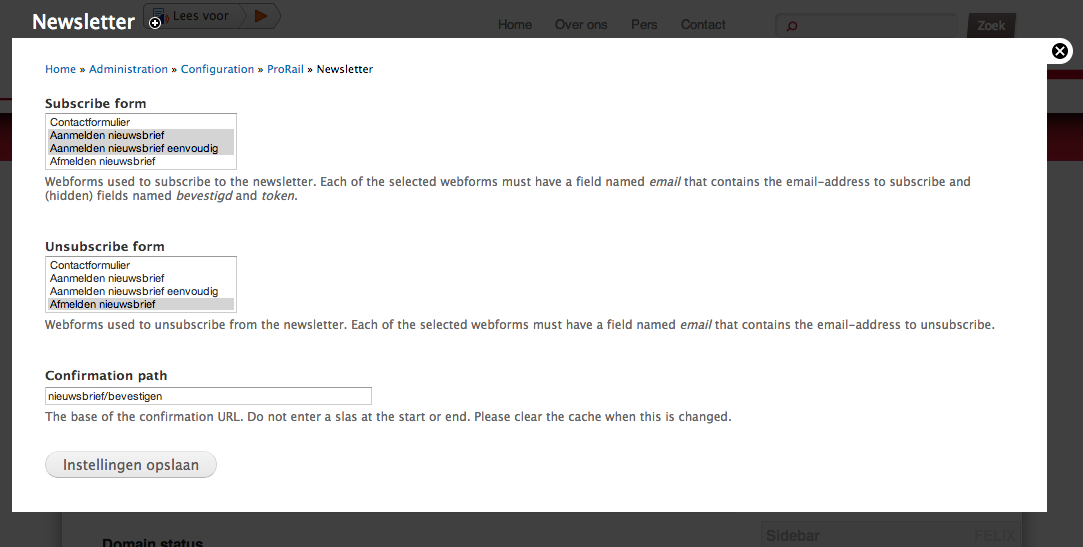
\includegraphics[width=\textwidth]{img/nieuwsbrief/nieuwsbrief_admin.png}
\end{figure}

\subsubsection{Vereisten afmeldformulieren}
\label{sec:vereistenafmeldformulieren}
De enige vereiste voor afmeldformulieren is dat ze een veld hebben met de 
machinenaam \emph{email} van het type \emph{email}. Extra velden kunnen naar 
eigen inzicht worden toegevoegd, bijvoorbeeld velden om een reden voor afmelding 
kenbaar te maken.

\subsubsection{Beheerinterface}
De beheer-interface van de module is te vinden onder Instellingen, ProRail, 
Newsletter.
De volgende instellingen zijn te maken:

\begin{itemize}
\item Het kiezen van webformulieren die dienst doen als aanmeldformulier (let op de vereisten 
zoals vermeld in \ref{sec:vereistenaanmeldformulieren}, of e.e.a. zal niet naar 
behoren werken).
\item Per aanmeldformulier een bijbehorend afmeldformulier (let op de vereisten 
zoals vermeld in \ref{sec:vereistenafmeldformulieren}).
\item Het instellen van het bevestigings-pad, dat wil zeggen de URL die de 
bevestigingen dient te verwerken. Dit is de link die vermeld dient te worden in de 
bevestigingsemail, die verantwoordelijk is voor het verwerken van aanmeldingstokens. 
Normaal gesproken hoeft dit niet aangepast te worden.
\end{itemize}

\subsubsection{Settings}

De module is instelbaar op admin/config/prorail/newsletter. Hier zijn de volgende zaken in te stellen:

\begin{enumerate}
\item Welke formulieren gelden als inschrijfformulier. Deze formulieren dienen een veld voor het email-adres te hebben met als sleutelveld 'email' en een tweetal verborgen velden, met de keys 'bevestigd' en 'token'. 'token' wordt bij indienen gevult met een unieke string, die in de bevestigingsemail wordt opgenomen in een link waarmee de aanmelding bevestigd moet worden (zie verder). 'bevestigd' wordt op 'ja' gezet zodra deze link bezocht is.

\item Welke formulieren gelden als afmeldformulier. Een email-adres ingevuld in het formulier-element met de sleutelveld 'email' heeft tot gevolg dat inzendingen van de aanmeldformulieren met dat email-adres worden verwijderd.

\item De basis voor bevestigings-URLs. Hier wordt het aangemaakte token aan vastgeplakt. Bijvoorbeeld: "nieuwsbrief/bevestigen". Het is van belang dat de URL die in de email wordt gezet hiermee overeenkomt. (Indien dit wordt verandert moet de cache gelegd worden omdat de menu router-tabel opnieuw opgebouwd moet worden).
\end{enumerate}

Voor de bevestigingsemail wordt de normale Webforms email-voorziening gebruikt. De bevestigingstoken is daar beschikbaar als value[token]. Dit is voor de huidige aanmeldformulieren al juist ingesteld.

\subsubsection{Formulieren nieuwsbrieven}

Een ingelogde gebruiker kan het formulier invullen. Er wordt dan geen e-mail verstuurd. Wel zie je de confirmatiepagina die reguliere gebruikers ook zien, waar staat dat er een e-mail is verstuurd (let dus op: dit gebeurt niet als je als content beheerder het formulier hebt ingevuld.).

Als ingelogde gebruiker kun je ook verplichte velden overslaan.

\begin{figure}[p]
\centering
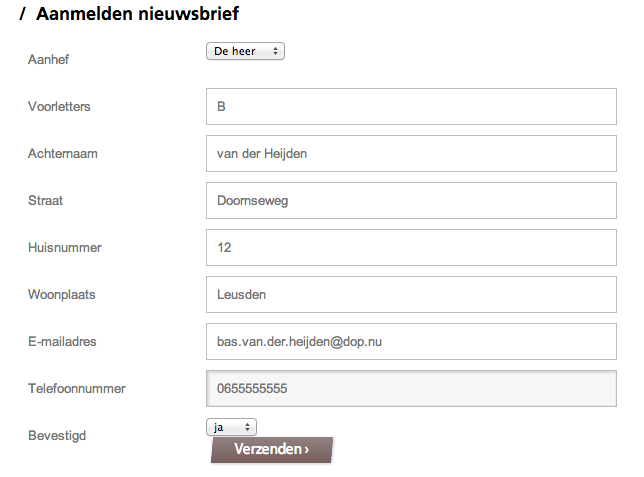
\includegraphics[width=\textwidth]{img/nieuwsbrief/nieuwsbrief_formulier.png}
\end{figure}


\subsection{Dominion}\label{dominion}
De \emph{Dominion} module wordt gebruikt voor het aanmaken van subsites. Ga naar \drupalpath{admin/structure/dominion} voor een overzicht van alle subsites. Het aanmaken van een subsite kan serveraanpassingen vereisen. Dit is zeker het geval wanneer een SSL certificaat op een van de (sub)sites actief is.

\bigskip

\begin{center}
	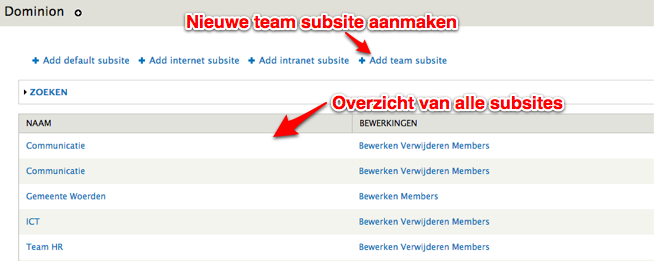
\includegraphics[width=\textwidth]{img/dominion1.png}
\end{center}

\subsubsection{Subsite toevoegen}\label{teamsubsitetoevoegen}
Klik op \emph{Add (internet/intranet/team) subsite} om een nieuwe subsite toe te voegen. 

Onder \emph{Domain type} staan maximaal drie keuzes. Niet alle keuzes kunnen actief zijn.

\begin{itemize}
\item Use a subdomein of .\drupalpath{}. Hiermee kan je subsites aanmaken waarvan de naam \emph{voor} het domein gezet worden. Dat kan dus \emph{intranet}.\drupalpath{} worden.
\item Use a custom domainname. Hier kan je een eigen domein opgeven die helemaal losstaat van het huidige domein. Let wel op dat hiervoor serveraanpassingen vereist zijn.
\item Use a directory. Hiermee kan je subsites aanmaken waarvan de naam \emph{achter} het domein gezet worden. Dat kan dus \drupalpath{}\emph{intranet} worden. Wanneer deze optie geselecteerd wordt zullen er een extra opties getoond worden. Kies bij \emph{Domein} voor het domein waar het achter moet komen. Kies bij \emph{Map} de url, in het voorbeeld zou dat dus \emph{intranet} zijn. 
\end{itemize}

\bigskip

\begin{enumerate}
\item Vul bij het veld \emph{Naam} een naam in voor de subsite.
\item Kies het juiste \emph{Domain type}.
\item Specificeer eventueel de overige opties.
\item Klik op de knop \emph{Opslaan} om de subsite toe te voegen .
\end{enumerate}

\bigskip

\begin{center}
	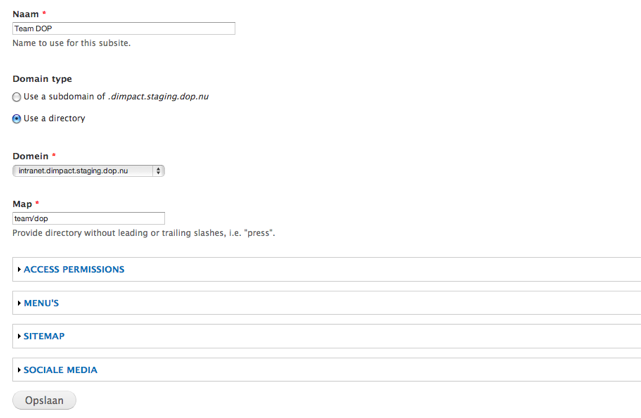
\includegraphics[width=\textwidth]{img/dominion2.png}
\end{center}

\subsubsection{Team members beheren}\label{teammembersbeheren}
Aan elke subsite kunnen \emph{Members} worden toegevoegd.

\bigskip

Klik op \emph{Members} bij de betreffende subsite om \emph{Members} toe te voegen.

\begin{center}
	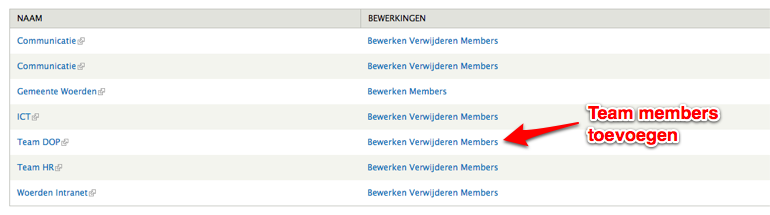
\includegraphics[width=\textwidth]{img/dominion3.png}
\end{center}

\bigskip
Op deze pagina is een lijst te vinden van de huidige teamleden.
Klik op "Add member" om een gebruiker aan de subsite toe te voegen.
Vul de gebruikersnaam of e-mail adres in, selecteer eventueel een domein specifieke rol (bijv. "teamlid") en klik vervolgens op de knop \emph{Toevoegen} om de gebruiker toe te voegen aan de lijst van \emph{Members}.

\bigskip

\begin{center}
	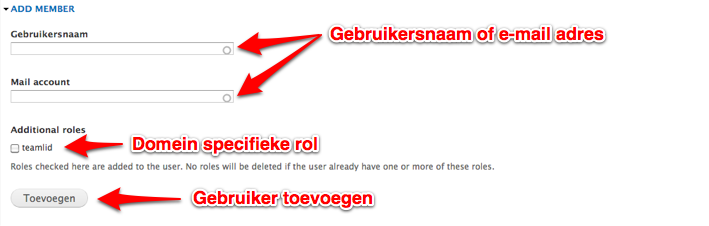
\includegraphics[width=\textwidth]{img/dominion4.png}
\end{center}


\subsection{Flexible blokken}\label{felix}
Het is voor redacteuren mogelijk om blokken de plaatsen op pagina's. Hiermee krijgt de redacteur enige vrijheid over de indeling van de pagina. Hier zijn wel beperkingen van toepassing volgens het grafisch ontwerp.

Door met de muis over de grijze balk te gaan verschijnt er een tandwieltje, als je daarop klikt dan verschijnt er een optie \emph{Blok toevoegen}. Hier kan een keuze gemaakt worden om een enkel item weer te geven op de website, dit zijn \emph{Nodetypes}, of een aantal items, zoals bijvoorbeeld \emph{Het laatste nieuws}.

\begin{center}
	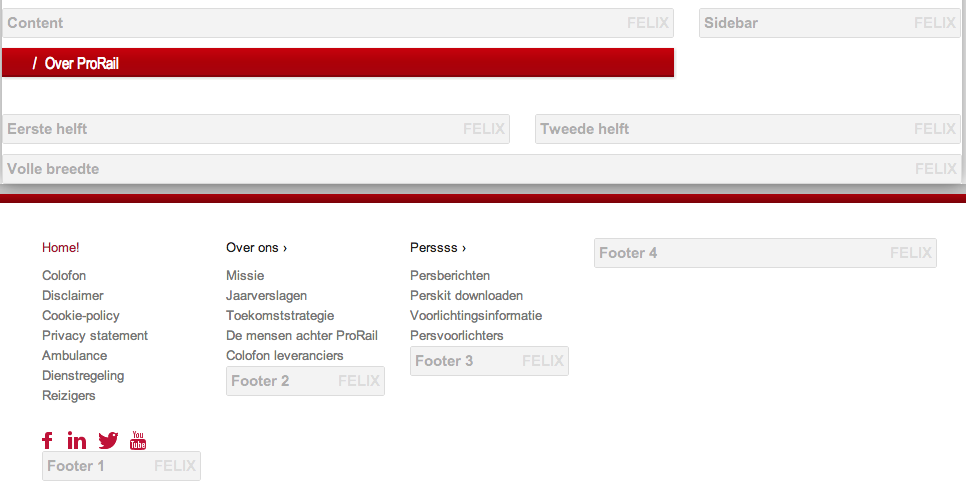
\includegraphics[width=\textwidth]{img/felix.png}
\end{center}
\subsection{Social media}

Ter ondersteuning van het delen op social media wordt voorzien in de volgende zaken:
\begin{itemize}
\item Share buttons
\item Mogelijkheid om widgets in HTML code te plaatsen
\item RSS feeds
\end{itemize}

\subsubsection{Share buttons}

De share buttons geven de mogelijkheid om de pagina te delen op de verschillende sociale media. Hierin kunnen de volgende buttons worden ingesteld:
\begin{itemize}
\item Facebook
\item Google+
\item LinkedIn
\item Twitter
\item Delen op Facebook (widget)
\item Twitteren (widget)
\end{itemize}

Bij oplevering van de standaarddistributie worden de specifieke share links aangezet. De widgets worden niet ingesteld. Deze kunnen bij implementatie van de gemeentesites makkelijk worden aangezet. De theming zal wel geschikt worden gemaakt voor het grotere formaat van deze widgets.

Buttons worden op alle nodetypes toegevoegd die een detailpagina hebben.

Per subsite wordt instelbaar of de share buttons direct zichtbaar zijn of onder een overlay komen. In het laatste geval is een enkele "delen" link beschikbaar waarmee de overlay geopend kan worden. Voor deze instelling wordt een custom \emph{dominion functie} aangemaakt met de systeemnaam \texttt{sharelink}. In het theme kan dan gebruik gemaakt worden van de functie \texttt{dominion\_has\_function} om te bepalen of de overlay gebruikt moet worden.

\subsubsection{Widgets in HTML-code}

Eindredacteuren krijgen de mogelijkheid om zelf HTML widgets te plaatsen in de body tekst\seeone{invoerformaten}.

\subsubsection{Externe RSS-feeds}

Via de \usemodule{views} module i.c.m. de \usemodule{views\_rss} module worden RSS feeds ingesteld. De volgende feeds worden aangemaakt:
\begin{enumerate}
\item Laatste nieuwsberichten
\item Actuele evenementen
\item Laatste bekendmakingen
\item Laatst gewijzigde pagina's
\end{enumerate}
De views worden gesorteerd op publicatiedatum (1 t/m 3) of datum laatst gewijzigd (4). De RSS feed laat altijd 20 items zien.

Nieuwe RSS feeds kunnen niet door de gemeente aangemaakt worden.


\subsection{Readspeaker}\label{readspeaker}

Voor de voorleesfunctie zullen we gebruikmaken van ReadSpeaker. De integratie hiervan gebeurt in het theme. Per gemeente wordt een apart account aangemaakt. Bij ReadSpeaker dienen hiervoor de relevante domeinen te worden ingesteld waarop deze actief wordt. De \emph{customer id} is nodig in Drupal.

In \texttt{page.tpl.php} wordt de volgende code gebruikt op de plaats waar de button moet komen:

\begin{lstlisting}[language=PHP]
  <?php $readspeaker_customerid = variable_get('readspeaker_customerid', 0); ?>
  <?php if ($readspeaker_customerid): ?>
  <div id="readspeaker_button1" class="rs_skip rsbtn rs_preserve">
    <a class="rsbtn_play" title="Laat de tekst voorlezen met ReadSpeaker" href="//app.eu.readspeaker.com/cgi-bin/rsent?customerid=<?php print $readspeaker_customerid; ?>&amp;lang=nl_nl&amp;readid=main&amp;url=<?php echo urlencode($_SERVER['HTTP_HOST'] . $_SERVER['REQUEST_URI']); ?>">
        <span class="rsbtn_left rsimg rspart"><span class="rsbtn_text"><span>Lees voor</span></span></span>
        <span class="rsbtn_right rsimg rsplay rspart"></span>
    </a>
  </div>
  <?php endif; ?>
\end{lstlisting}

In \texttt{html.tpl.php} wordt de volgende code gezet binnen de \texttt{\textless head\textgreater}:
\begin{lstlisting}[language=PHP]
<script src="<?php print base_path() . path_to_theme() . '/readspeaker/ReadSpeaker.js?pids=embhl'; ?>"></script>
\end{lstlisting}

De JavaScripts van readspeaker worden zelf gehost en dus ook in het theme gezet. Dat is nodig om de button te laten werken op SSL.

De \emph{customer id} kan worden ingesteld in \texttt{settings.php}:
\begin{lstlisting}[language=PHP]
$conf['readspeaker_customerid] = 1234;
\end{lstlisting}

Wanneer deze niet gezet is zal de button niet worden getoond.
\subsection{Google Analytics}\label{googleanalytics}
De bezoekersstatistieken van de \drupalpath website en haar subsites worden bijgehouden d.m.v. Google Analytics. Het \emph{Intranet} wordt bijgehouden door \emph{Piwik}.

De module \emph{Googleanalytics}  wordt gebruikt voor het koppelen van je Google Analytics account. Ga naar \drupalpath{admin/config/system/googleanalytics} om uw Google Analytics account te kopellen aan Dimpact. 

Vul bij het veld \emph{Web Property ID} je eigen Google ID code in. 

Klik vervolgens onderaan de pagina op de knop \emph{Instellingen opslaan} om de instellingen op te slaan.
\subsection{Piwik statistieken}\label{piwikstatistieken}
Statistieken van het \emph{Intranet} worden bijgehouden d.m.v. \emph{Piwik}. 
Je kunt via \drupalpath{admin/config/system/piwik} de module instellen. De onderstaande afbeelding legt uit hoe dit moet. 

Op piwik.\drupalpath kun je de statistieken bekijken, je dient wel met een bevoegde gebruiker te zijn ingelogd. 

\begin{center}
	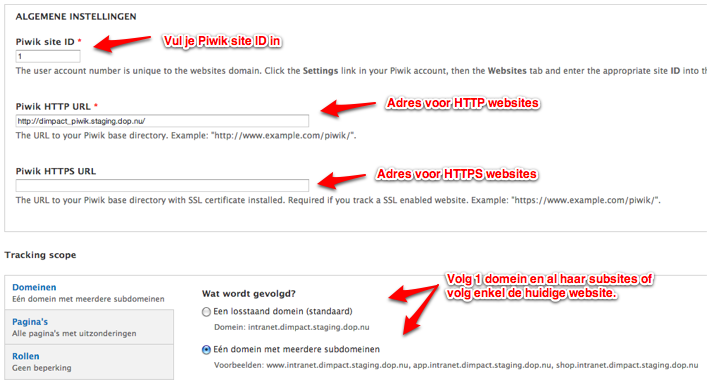
\includegraphics[width=\textwidth]{img/piwik.png}
\end{center}
\subsection{Sitemap}\label{sitemap}
De sitemap wordt standaard ingesteld tijdens de installatie van Dimpact. Mocht je de sitemap toch naar wens willen aanpassen dan kun je dit doen via de volgende link: \drupalpath{admin/config/search/sitemap}

In dit formulier kun je aangeven wat er in de sitemap moet komen te staan. Voer bij \emph{Paginatitel} een titel voor de pagina in. Onder \emph{Sitemap bericht} kan je een tekst plaatsen die op de pagina zichtbaar is. 

Onder \emph{SITEMAP INHOUD} kan je kiezen voor de volgende instellingen. \emph{Geef de voorpagina weer}, plaats een link naar de voorpagina. \emph{Menu's die in de sitemap moeten worden opgenomen}, geef aan welke menu's getoond moeten worden als lijstweergave op de sitemap. \emph{Geef FAQ inhoud weer}, toont een lijst met FAQ items. \emph{Categorieen die in de sitemap moeten worden opgenomen}, toont een lijst met taxonomietermen die binnen de vocabulaires vallen.

Onder \emph{CATEGORIE-INSTELLINGEN} stel je de weergavemodus in voor de te tonen taxonomietermen. \emph{Show node counts by categories} toont het aantal gekoppelde nodes aan een taxonomieterm. \emph{Categories depth} geef de diepte op tot op welk niveau termen opgehaald moeten worden. \emph{thresholds} geven aan vanaf hoeveel gekoppelde items de term weergegeven moet worden.

Onder \emph{RSS-INSTELLINGEN} stel je de instellingen in voor de RSS feed. Onder \emph{CSS SETTINGS} kan je opgeven of je het CSS bestand bij de RSS feed wilt inladen.

Klik onderaan de pagina op de knop \emph{Instellingen opslaan} om te instellingen op te slaan. De sitemap wordt dan beschikbaar op /sitemap.
\subsection{Cache}\label{cache}
\emph{Drupal} maakt gebruik van \emph{caching} functionaliteit. Het doel van \emph{caching} is de website sneller maken. De cache slaat bijvoorbeeld pagina's op in de database. Op deze manier kan de website, gebruikmakend van de cache, de al eerder opgeslagen pagina een stuk sneller tonen. 

Na het wijzigen van bijvoorbeeld content of menu-items moet de cache handmatig verschoont worden, indien je de wijzigingen \emph{direct} zichtbaar wilt maken. 

\textbf{Cache opschonen:}

\begin{enumerate}
\item Ga naar  \drupalpath{admin/config/development/performance}
\item Klik op de knop \emph{Alle caches legen}
\item Wacht op de succes melding, dit duurt ongeveer een halve minuut
\end{enumerate}

\begin{center}
	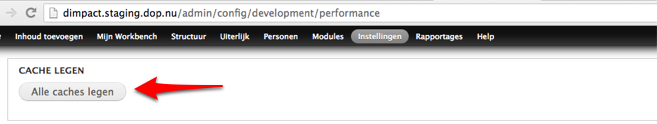
\includegraphics[width=\textwidth]{img/cache.png}
\end{center}
\subsection{Cookiebalk}\label{cookiebalk}
De instellingen van deze module zijn te vinden op: \drupalpath{admin/config/user-interface/cookie-consent}. De volgende instellingen kunnen worden aangepast:

\begin{itemize}
\item \emph{More information Node Link}. Vul hier de titel van de node in waar de informatie over het cookiegebruik van de website op staat.
\item \emph{More information Link Title}. Vul hier de tekst van de meer informatie-knop in.
\item \emph{Rolen}. De rollen die de cookiebalk te zien krijgen.
\item \emph{Exclude Cookie Consent}. Vul hier de paden van pagina's in waarop de cookiebalk niet te zien mag zijn.
\item \emph{Exclude Domains}. Selecteer domeinen waarop de cookiebalk niet te zien mag zijn.
\item \emph{Cookie Consent Style}. Bepaal het uiterlijk van de balk. Dit kan licht, donker of monochrome (zwart/wit) zijn.
\item \emph{Hide the privacy tab}. Verberg het tabblad.
\item \emph{Privacy Tab Position}. Plaats van het tabblad op in het browserscherm.
\item \emph{Banner position}. De positie van de cookiebalk.
\item \emph{Refresh on consent}. Ververs de pagina wanneer de gebruiker akkoord heeft gegeven op het gebruik van cookies. 
\item \emph{Filter iframe tags}. Toon geen inhoud van iframes zolang er geen akkoord is gegeven op het gebruik van cookies.
\item \emph{Stricly necessary Scripts}, \emph{Social Media Scripts}, \emph{Advertising Scripts}, \emph{Analytics Scripts}. Hier kunnen scripts worden opgevoerd die uitgevoerd moeten worden na akkoord.
\end{itemize}
\subsection{Forum}\label{forum}
Te vinden op \drupalpath{forum}.

\subsubsection{Aanmaken forumcategorieen}\label{forumcategorieen}
Op \drupalpath{admin/structure/taxonomy/forums} zijn forumonderwerpen aan te maken. Dit zijn de onderwerpen op het hoogste niveau binnen het forum. Voor de onderwerpen worden taxonomietermen gebruik.

\subsubsection{Aanmaken forumonderwerpen}\label{forumonderwerpen}
Het aanmaken van een nieuw forumonderwerp doe je door op de knop \emph{Forumonderwerp toevoegen} te drukken. Hierna volgt een itembewerkpagina waar je het onderwerp kan aanmaken. Selecteer een forumcategorie (Forums) om het onderwerp in een van de categorieen te plaatsen. Maak je een nieuw onderwerp aan binnen een categorie zal deze automatisch geselecteerd zijn.

\begin{center}
	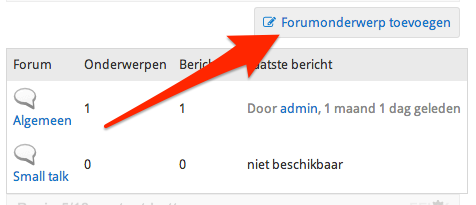
\includegraphics[width=\textwidth]{img/forumonderwerp.png}
\end{center}
\subsection{Redirects}\label{redirects}
Het is mogelijk binnen de website redirects aan te maken, waardoor de bezoeker vanaf een bepaald URL kan worden doorverwezen naar een ander URL. Dit is bijvoorbeeld nuttig wanneer een pagina is verhuisd, en een bezoeker het oude URL nog in de bookmarks kan hebben staan.

\textbf{Redirect aanmaken}

\begin{itemize}
\item Ga naar \emph{/admin/config/search/redirect}
\item Klik op \emph{Add redirect}
\item Voer bij \emph{van} en URL in vanaf waar de bezoeker moet worden doorverwezen
\item Voer bij \emph{naar} het URL in waar de bezoeker naar toe moet worden geleid.
\item Wijzig eventueel de HTTP-code onder de uitgebreide opties. Standaard staat deze op 301, wat wordt gebruikt wanneer een pagina permanent is verhuisd.
\end{itemize}

\subsection{Huisstijl kleuren}

De kleuren van de huisstijl kunnen door beheerders worden aangepast. Ga naar \emph{Uiterlijk} en klik op de link \emph{Instelingen} bij het thema \emph{Dimpact} of ga direct naar \drupalpath{admin/appearance/settings/dimpact}.

Op deze pagina staat een dropdown waarmee vooraf instelde kleurcombinaties gekozen kunnen worden. Het is ook mogelijk om zelf kleuren in te stellen a.d.v. de kleurcode (hexadecimaal) of color picker. Klik onderaan op \emph{Instellingen opslaan} om de wijzigingen door te voeren. De wijzigingen zijn direct actief.

\subsection{Custom CSS}\label{custom css}
De weergave van elementen kan worden aangepast door een custom CSS-bestand te uploaden. Let er op dat het toevoegen van een custom CSS mogelijk negatieve gevolgen heeft voor de bestaande weergave van elementen op de website.

\textbf{CSS uploaden}

\begin{itemize}
\item Ga naar \emph{/admin/appearance/css}
\item Kies \emph{choose file} bij het medium waarvoor de CSS moet worden aangepast
\item Upload een CSS bestand
\end{itemize}

Bij het uploaden van een lettertype is de gemeente verantwoordelijk voor aanschaf van de bijhorende weblicentie, wanneer van toepassing. Het Dimpact-moedersjabloon voorziet niet in licenties voor custom fonts.